Until now, I haven't been explicit about my definition of ``signal.''
Ultimately, $\Gamma_{ee}$ will be derived from the total integrated
$\Upsilon$ cross-section, so in that sense, every $\Upsilon$ decay is
my signal.  However, leptonic final states ($e^+e^-$, $\mu^+\mu^-$,
and $\tau^+\tau^-$, but not cascades that might contain leptons)
should be suppressed to avoid large continuum subtractions and
possible systematics due to interference with these modes.  In fact,
the quantity which is most often quoted in place of $\Gamma_{ee}$ is
$\Gamma_{ee}\Gamma_\subs{had}/\Gamma_\subs{tot}$, which is derived
from the integrated hadronic cross-section.  (Here, ``hadronic
cross-section'' means all modes other than leptonic final states.)

To translate from $\Gamma_{ee}\Gamma_\subs{had}/\Gamma_\subs{tot}$ to
$\Gamma_{ee}$, one multiplies by a factor of
\begin{equation}
  \frac{\Gamma_\subs{tot}}{\Gamma_\subs{had}} = \frac{1}{1 - 3
  \mathcal{B}_{\mu\mu}}  \mbox{ (assuming lepton universality).}
\end{equation}
This process is exactly the same as defining all $\Upsilon$ decays as
the signal and using Monte Carlo to correct for missing leptonic
modes.  Nevertheless, I'm going to stick with tradition and define all
non-leptonic decay modes of $\Upsilon$ to be my signal, and $\Upsilon
\to e^+e^-$, $\mu^+\mu^-$ as backgrounds.  The third leptonic mode,
$\Upsilon \to \tau^+\tau^-$, is 57\% efficient for the cuts that
define event type hadron.  It could therefore be considered a large
background, but it {\it is} part of what I will be adding back in
later.  Furthermore, I can't simply subtract it, as it has complicated
interference behavior through the resonance scan.  I treat it,
therefore, as a second signal.

I do not often make this distinction between signal and leptonic modes
in comparisons of data and Monte Carlo.  In comparing two histograms, I
could leave the leptons in the data and in the Monte Carlo, or I could
use the Monte Carlo to subtract them from the data.  Both of these
result in exactly the same comparison.  Therefore, I will usually
leave the leptons in the data when I am only comparing with Monte
Carlo.  (The only place in this paper where I did remove leptons from
data is in Subsection \ref{trigger:subsection_lowlevel}.)

\section{Measurement Technique}

My technique for measuring hadronic efficiencies will be as follows.
\begin{enumerate}

  \item Trigger: I have set a 0.66\%, 1.04\%, 1.04\% error on the
    Monte Carlo's estimate of this (which is essentially 100\%).

  \item \dxy: The cascades study tells me that I can trust the Monte
    Carlo for this cut, within 0.15\% ``validity uncertainty.''  (See
    Table \ref{cascades_contributions}.)  The looseness of this cut
    suggests that I can apply the same 0.15\% to the $\Upsilon(2S)$
    and $\Upsilon(3S)$.

  \item \dz: Same thing except that the validity uncertainty is
    0.48\%.

  \item \pone: The validity uncertainty is 0.35\% for hadronic decays.
    This cut strongly discriminates between cascades to leptons and
    all other hadronic decays, so I will want to break the Monte Carlo
    up into different modes and propagate uncertainties from branching
    fractions.

  \item \visen: Limitations in the cascades study prohibit me from
    applying the same technique.  I instead add a cascades
    measurement of very low visible energy (0--30\% \ecom) to an
    unfiltered-dataset measurement of low visible energy (30--40\%
    \ecom) for a total cut efficiency.

  \item \lfourdec: This is highly efficient after all cuts, so I
    simply count surviving events from the unfiltered dataset.

\end{enumerate}

After visually checking for data/Monte Carlo discrepancies, I will
read off the efficiency of cuts \#1--\#4 from Monte Carlo, vary
branching fractions in the Monte Carlo, and then add to the error the
validity uncertainties I determined from cascades.  The efficiency of
the \visen\ cut given \#1--\#4 will be measured using the
cascades+unfiltered data technique, and then multiplied for the total
efficiency of cuts \#1--\#5.  Then I will use the data to show that
the last cut has negligible impact.

This means that I am not a priori trusting the Monte Carlo.  The
$\Upsilon(1S)$ efficiency doesn't really depend on the Monte Carlo at
all: the validity uncertainties derived from the cascades study is the
difference between the true efficiency and the Monte Carlo's estimate.
Likewise, all hadronic decay modes shared by the $\Upsilon(2S)$ and
$\Upsilon(3S)$ ($ggg$, $gg\gamma$, and $q\bar{q}$) are actually tied
to the true $\Upsilon(1S)$ efficiency through these validity
uncertainties.  My assumption is that the $\Upsilon(1S)$ efficiencies
apply to the $\Upsilon(2S)$ and $\Upsilon(3S)$ for non-cascade decays.
For cascade decays, however, I am trusting the Monte Carlo: in
principle, the true $\chi_b$ efficiency might be very different from
the Monte Carlo's estimate.  But I assume that because the Monte Carlo
has successfully reproduced $ggg$ hadronization, it will also
correctly reproduce $gg$ hadronization.

I explicitly trust the Monte Carlo's prediction of all leptonic
efficiencies, including the mode $\Upsilon \to \tau^+\tau^-$.  Only
branching fraction uncertainties are propagated.
 
\section{Overlays of Unfiltered Data and Monte Carlo}

Monte Carlo simulations of $\Upsilon(1S)$ decays were shown to be
consistent with the data in cascade decays, but its validity for
direct $\Upsilon(1S)$ production or for the $\Upsilon(2S)$ or
$\Upsilon(3S)$ has yet to be seen.

Overlays of unfiltered data and Monte Carlo are presented in Figures
\ref{efficiency_dxy}, \ref{efficiency_dz}, \ref{efficiency_p1}, and
\ref{efficiency_visen}.  Cuts were applied cumulatively, so the first
two (\dxy\ and \dz) are significantly distorted by backgrounds.
(Continuum, beam-gas, and cosmic rays have all been subtracted, but
\dxy\ and \dz\ aren't perfectly represented by the single- and no-beam
samples.)  That is why these first two cuts are very loose: to bolster
confidence in the predicted efficiency of the cut in the face of large
backgrounds.  Only special classes of signal events which vertex far
from the origin wouldn't be visible in these plots, but the cascades
study would have caught this possibility.  (The ``validity
uncertainties'' are upper limits on these branching fractions.)

\begin{figure}
  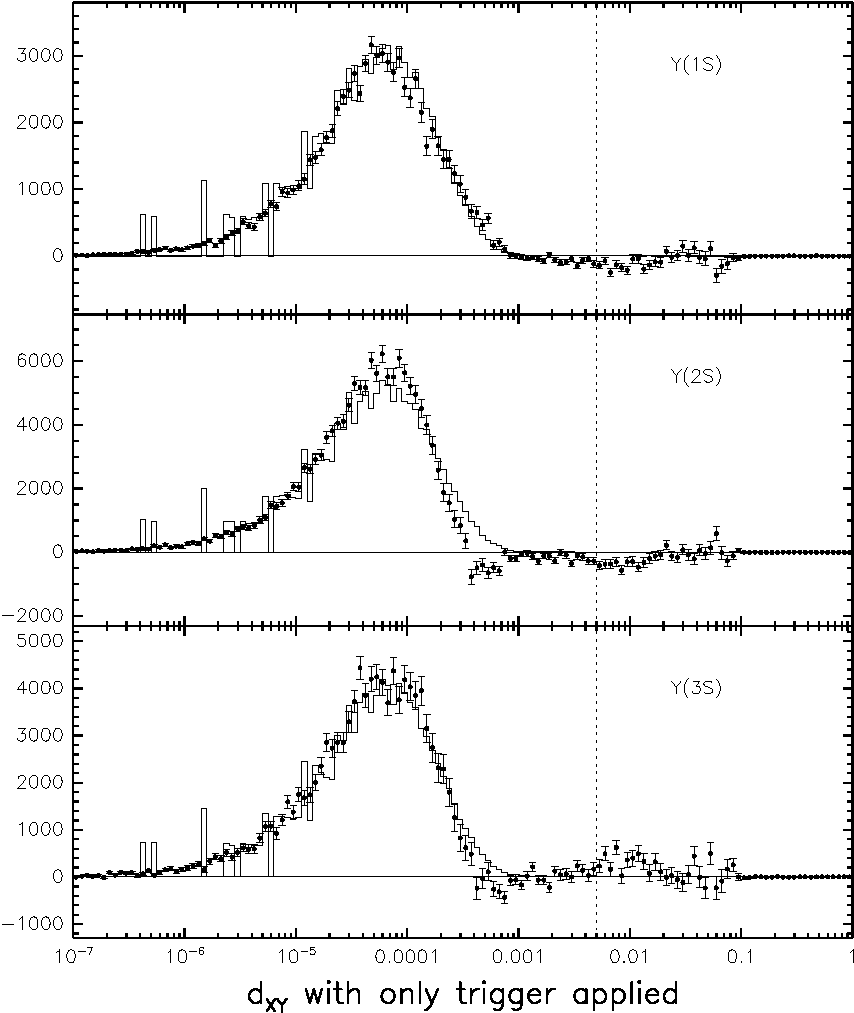
\includegraphics[width=\linewidth]{plots/efficiency_dxy}
  \caption{\label{efficiency_dxy} Closest track to the beamspot in XY,
    presented in log $x$ scale, for the three resonances (data with
    errorbars), compared with Monte Carlo (solid histogram).  The cut
    boundary is indicated by the dotted line.}
\end{figure}

\begin{figure}
  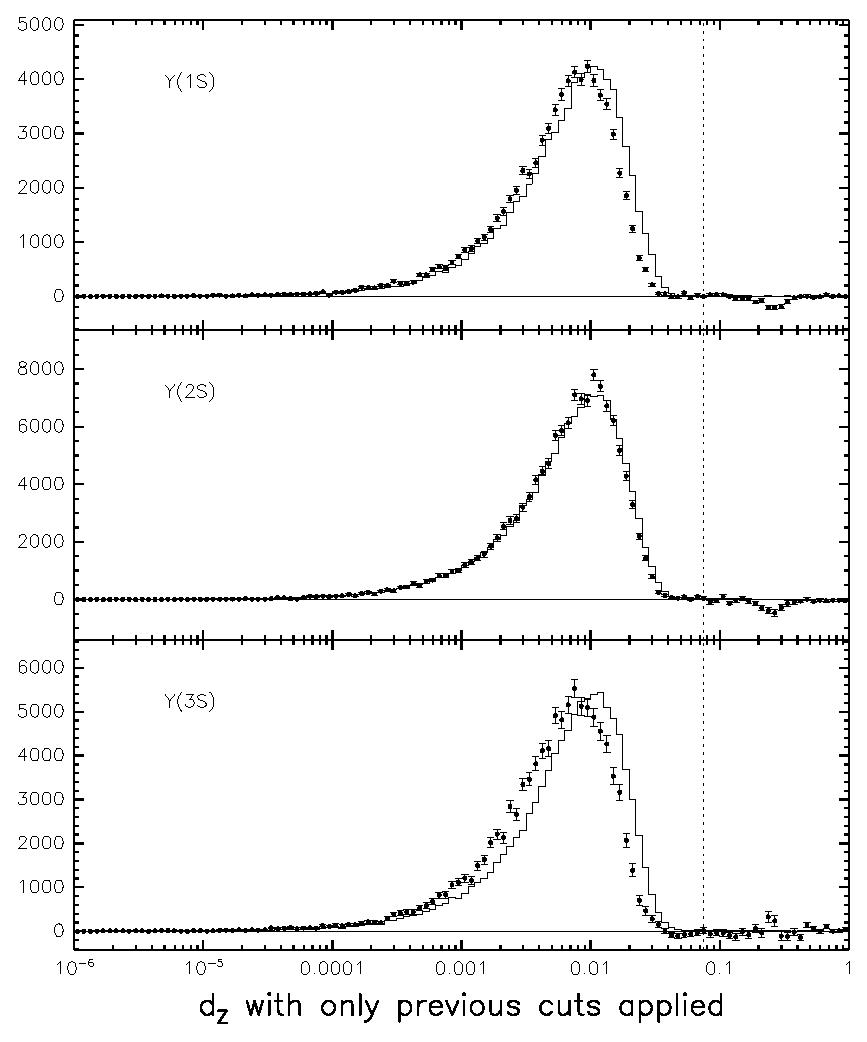
\includegraphics[width=\linewidth]{plots/efficiency_dz}
  \caption{\label{efficiency_dz} Event vertex Z, presented in log $x$
    scale, for the three resonances (data with errorbars), compared
    with Monte Carlo (solid histogram).  The cut boundary is indicated
    by the dotted line.}
\end{figure}

\begin{figure}
  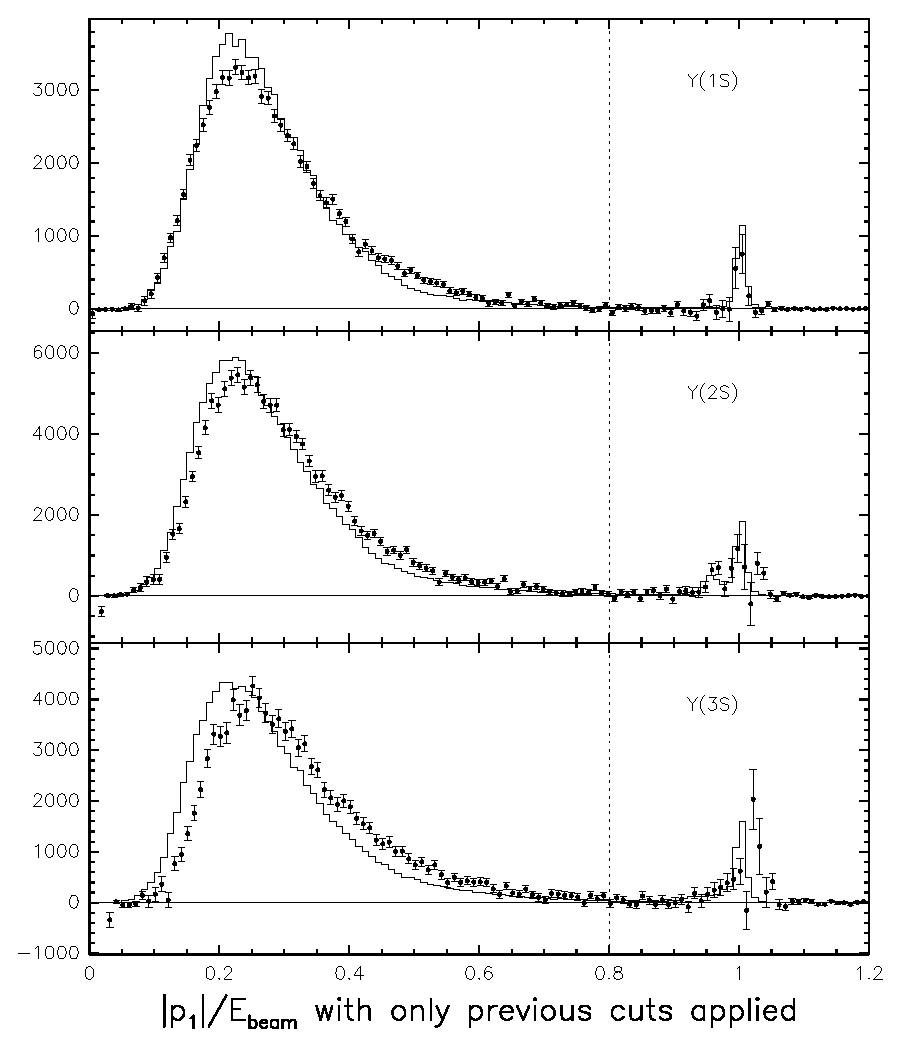
\includegraphics[width=\linewidth]{plots/efficiency_p1}
  \caption{\label{efficiency_p1} Largest track momentum divided by
    \ebeam\ for the three resonances (data with errorbars), compared
    with Monte Carlo (solid histogram).  The cut boundary is indicated
    by the dotted line.}
\end{figure}

\begin{figure}
  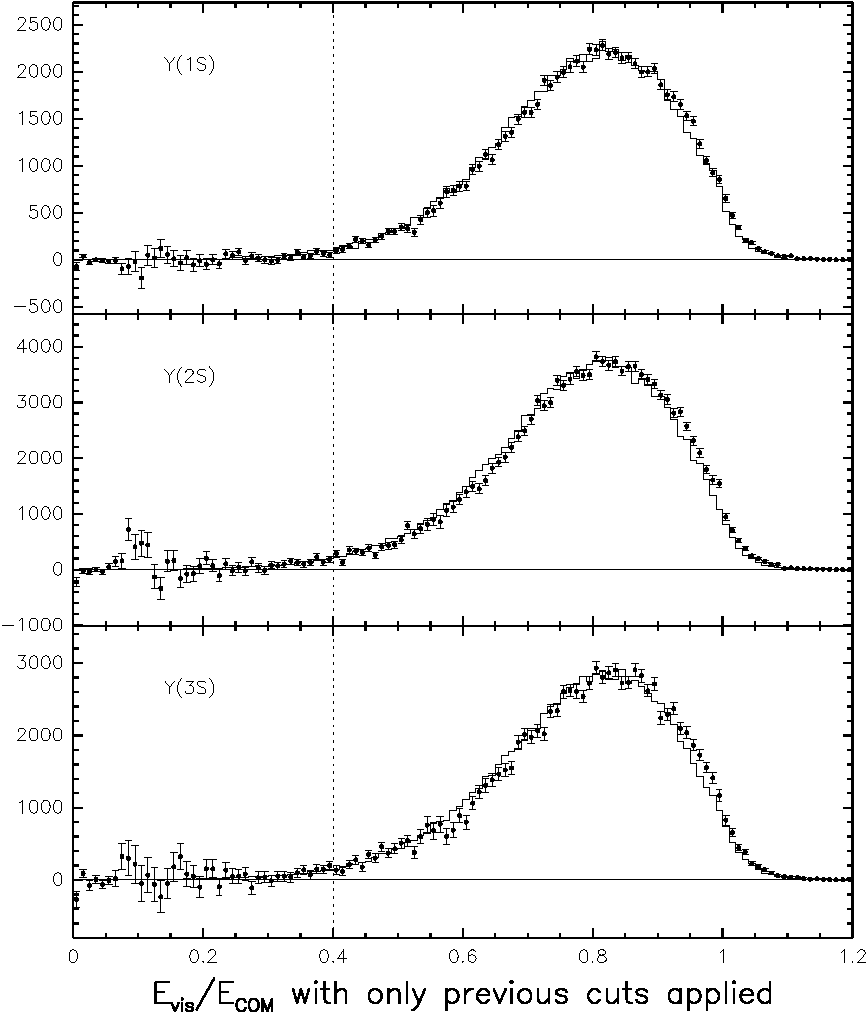
\includegraphics[width=\linewidth]{plots/efficiency_visen}
  \caption{\label{efficiency_visen} Visible energy divided by \ecom\
    for the three resonances (data with errorbars), compared with
    Monte Carlo (solid histogram).  The cut boundary is indicated by
    the dotted line.}
\end{figure}

The third and fourth cuts, \pone\ and \visen, are much tighter, but
can be observed in a low-background environment.  The difference in
the shape of \pone\ from 10\% to 60\% \ebeam\ between data and Monte
Carlo is disturbing.  But it is present in the $\Upsilon(1S)$, and can
even be seen in cascade plots (Figure \ref{cascades_p1}), and yet the
data/Monte Carlo difference is only 0.35\%.  In Figure
\ref{efficiency_overlay}, we see that the three resonances don't seem
to differ in the tail, so the 0.35\% applies to each.  Also in Figure
\ref{efficiency_overlay}, we see that the three resonances have very
similar \visen\ distributions, so they can share a visible energy
correction.

\begin{figure}
  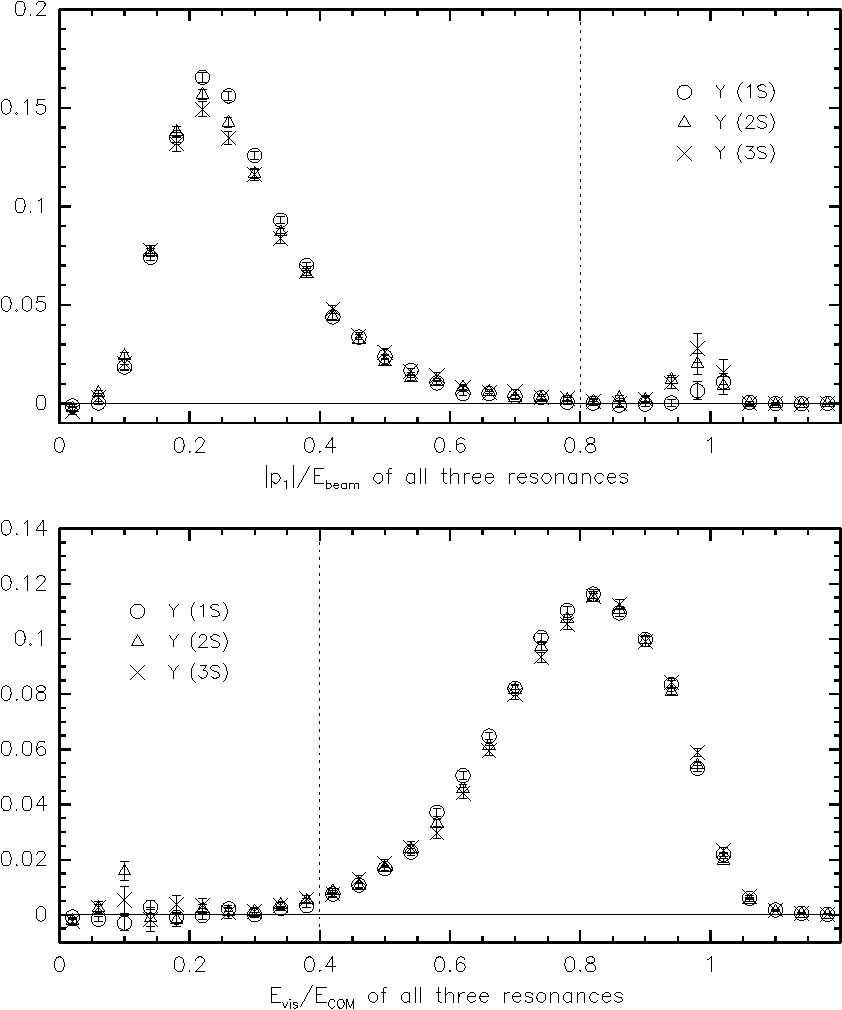
\includegraphics[width=\linewidth]{plots/efficiency_overlay}
  \caption{\label{efficiency_overlay} Largest track momentum (as a
  fraction of \ebeam) and visible energy (as a fraction of \ecom) for
  all three resonances overlaid upon each other, rather than the
  Monte Carlo.  Cut boundaries are indicated by the dotted lines.}
\end{figure}

\section{Cut Efficiencies from Monte Carlo}

The only cut efficiency that will be measured using signal Monte Carlo
is the combination of cuts \#1--\#4 (trigger through \pone).  With the
exception of $\tau^+\tau^-$, all modes are either very efficient or
very inefficient.  This will trivialize the Monte Carlo's dependence
on variations in branching fractions.  The mode-by-mode efficiencies
are listed in Table \ref{efficiency_montecarlo}, and the aggregate
efficiency in Table \ref{efficiency_montecarlo3}.

I used the following to combine the individual mode efficiencies:
\begin{eqnarray}
  \mathcal{B}_{q\bar{q}} &=& R \mbox{ } \mathcal{B}_{\mu\mu} \\
  \mathcal{B}_{\mbox{\scriptsize cascades}} &=& 0 \mbox{ } (1S), \mbox{\hspace{0.25 cm}} 45.4 \pm 1.5\% \mbox{ } (2S), \mbox{\hspace{0.25 cm}} 45.2 \pm 1.5\% \mbox{ } (3S) \\
  \mathcal{B}_{ggg} &=& \frac{1 - (3+R)\mathcal{B}_{\mu\mu} - \mathcal{B}_{\mbox{\scriptsize cascades}}}{1 + \Gamma_{gg\gamma / ggg}} \\
  \mathcal{B}_{gg\gamma} &=& (\Gamma_{gg\gamma/ggg}) \, \mathcal{B}_{ggg}
\end{eqnarray}
The leptonic branching fraction $\mathcal{B}_{\mu\mu}$ was measured to
high precision recently by Istvan Danko, with the values 2.49 $\pm$
0.07\% ($\Upsilon(1S)$), 2.03 $\pm$ 0.09\% ($\Upsilon(2S)$), and 2.39
$\pm$ 0.12\% ($\Upsilon(3S)$) [\ref{cite:istvan}].  The ratio of quark
pairs to muon pairs, $R$, is 3.58 $\pm$ 0.14 [\ref{cite:novoR}].  For
cascade branching fractions, I added together all cascade modes in the
PDG [\ref{cite:pdg}].

There seems to be a discrepancy in the literature regarding the value
of $\Gamma_{gg\gamma}/\Gamma_{ggg}$; a direct measurement
[\ref{cite:cleoggg}] yields 2.75\% $\pm$ 0.16\% and the world-average
of $\alpha_s$ run to $M_\Upsilon$ predicts a value of 3.65\% $\pm$
0.05\% [\ref{cite:pdgggg}], using the formula
\begin{equation}
\frac{\Gamma_{gg\gamma}}{\Gamma_{ggg}} = \frac{36 \, {e_b}^2}{5} \frac{\alpha_{QED}}{\alpha_s(M_\Upsilon)}
\left( 1 + 2.2(6) \, \frac{\alpha_s(M_\Upsilon)}{\pi} + \mbox{\ldots} \right) \mbox{.}
\end{equation}
My value, 3.20 $\pm$ 0.45\%, straddles these two, with an error
large enough to encompass both.

It matters very little what value I use, since the aggregate
efficiency is insensitive to all cut variations, as seen in Table
\ref{efficiency_montecarlo2}.  Included in this table is sensitivity
to a known bug in my Monte Carlo sample (I toggle between unaffected
and all events), sensitivity to code release (the same events were
processed in different code releases), and the statistical error in
the Monte Carlo sample.

\begin{table}[t]
  \caption{\label{efficiency_montecarlo} Monte Carlo efficiencies for
    each mode for cuts \#1--\#4 (up to and including \pone)}
  \begin{center}
    \begin{tabular}{l c c c}
       & $\Upsilon(1S)$ & $\Upsilon(2S)$ & $\Upsilon(3S)$ \\\hline
      $e^+e^-$ & 0.24\% & 0.23\% & 0.28\% \\
      $\mu^+\mu^-$ & 0.16\% & 0.13\% & 0.19\% \\
      $\tau^+\tau^-$ & 77.25\% & 78.66\% & 77.03\% \\
      $ggg$ & 99.75\% & 99.78\% & 99.78\% \\
      $gg\gamma$ & 96.44\% & 96.69\% & 96.44\% \\
      $q\bar{q}$ & 97.99\% & 98.20\% & 98.37\% \\
      cascade $\to e^+e^-$ or $\mu^+\mu^-$ & & 0.90\% & 0.76\% \\
      cascade $\to$ other modes & & 99.53\% & 99.48\% \\
    \end{tabular}
  \end{center}
\end{table}

\begin{table}[p]
  \caption{\label{efficiency_montecarlo3} Aggregate hadronic Monte
    Carlo efficiency for cuts \#1--\#4 (up to and including \pone)}
  \begin{center}
    \begin{tabular}{l c c c}
       & $\Upsilon(1S)$ & $\Upsilon(2S)$ & $\Upsilon(3S)$ \\\hline
      Hadronic efficiency of cuts \#1--\#4 & 99.52\% & 97.92\% & 98.19\% \\
    \end{tabular}
  \end{center}
\end{table}

\begin{table}[p]
  \caption{\label{efficiency_montecarlo2} Hadronic Monte Carlo
    sensitivity to variations in branching fractions and other
    parameters}
  \begin{center}
    \begin{tabular}{l c c c}
       & $\Upsilon(1S)$ & $\Upsilon(2S)$ & $\Upsilon(3S)$ \\\hline
      $\mathcal{B}_{\mu\mu}$ (affects $q\bar{q}$ fraction) & 0.006\% & 0.010\% & 0.012\% \\
      $R$ (affects $q\bar{q}$ fraction)                    & 0.005\% & 0.005\% & 0.005\% \\
      $gg\gamma/ggg$                                       & 0.013\% & 0.006\% & 0.006\% \\
      $\mathcal{B}_\subs{cascades}$                        &         & 0.054\% & 0.044\% \\
      $\mathcal{B}_{ee}$ and $\mathcal{B}_{\mu\mu}$ of lower resonances &         & 0.003\% & 0.003\% \\\hline
      Bunch-finder bug                                      & 0.28\%  & 0.33\%  & 0.19\% \\
      Code release                                         & 0.011\% & 0.002\% & \\
      Finite sample                                        & 0.43\%  & 0.31\%  & 0.31\% \\\hline
      Sum in quadrature                                    & 0.51\%  & 0.46\%  & 0.37\% \\
    \end{tabular}
  \end{center}
\end{table}

\section{Cut Efficiencies from Unfiltered Data}

As can be seen in Figure \ref{efficiency_visen}, there is a great
uncertainty in the 0--30\% \ecom\ region of \visen, because a large
continuum peak is being subtracted there.  This uncertainty is all the
more acute since it is unclear what scale factor $S_c$ to use to
subtract these events, as many of them may be two-photon.  The region
from 30\% to 40\% \ecom\ is less uncertain, and it is here that signal
efficiency begins.  That is why I will measure only this part of the
\visen\ cut efficiency in the unfiltered dataset, leaving the rest for
the cascade dataset, which has substantially less background.

Why not measure the entire cut with cascades?  For one thing, I am
concerned about accepting a 1\% correction to $\Gamma_{ee}$ without
testing it in a non-boosted, $\pi^+\pi^-$-free environment.  Most of
the signal events that fail the \visen\ cut are in the 30--40\% \ecom\
region, so they are accessible to the unfiltered dataset.  By
splitting the measurement into two parts, I obtain a correction which
is consistent with zero from the cascades and a significant correction
from the unfiltered dataset.

The 30--40\% \ecom\ region accounts for 0.52 $\pm$ 0.12\% of the
events in the $\Upsilon(1S)$ plot, 1.01 $\pm$ 0.14\% of the events in
the $\Upsilon(2S)$ plot, and 0.85 $\pm$ 0.21\% of the events in the
$\Upsilon(3S)$ plot.  Toggling cosmic ray and beam-gas backgrounds
only changes the results by 0.01\%, 0.02\%, and 0.10\%, respectively.

Nor is there a significant dependence on ``database partition.''  Most
calibrations are applied to month-long sets of runs called database
partitions: $\Upsilon(3S)$ is split into db16 and db17 (a small part
is in db22, but the unfiltered dataset doesn't include any of these
runs), $\Upsilon(1S)$ is split into db18 and db19 (a small part is in
db17, but again, the unfiltered dataset doesn't include any such
runs), and $\Upsilon(2S)$ is split between db21, db22, db23, db25, and
db27 (the unfiltered dataset distinguishes between runs from db21 and
runs from db23, db25, and db27).  The efficiencies differ between
datasets by 0.22\%, 0.18\%, and 0.25\% for the $\Upsilon(1S)$,
$\Upsilon(2S)$, and $\Upsilon(3S)$.

Another source of systematic error is the fact that the continuum
scale factor, $S_c$, can vary through the plot.  Where the continuum
is dominated by two-photon events, the continuum subtraction should
use 1.005 $\times$ $S_c$, and where it is dominated by everything
else, the continuum subtraction should use $S_c$ as it was calculated
in Chapter \ref{chp:datasets}.  Taking an extreme case, I used 1.005
$\times$ $S_c$ in the 30--40\% \ecom\ region and $S_c$ everywhere
else.  The measurement changed by 0.02\%, 0.05\%, and 0.10\% for
$\Upsilon(1S)$, $\Upsilon(2S)$, and $\Upsilon(3S)$, respectively.

These systematic errors are listed and combined in Table
\ref{efficiency_datapart}.  A branching fraction to events with
\visen\ less than 40\% was obtained by adding the unfiltered dataset
result (30--40\%) to the cascades dataset (0--30\%).  The \visen\ cut
efficiency is the compliment of this.

\begin{table}[t]
  \caption{\label{efficiency_datapart} Summary of the \visen\ cut
    measurement.  Arrows indicate a result from one resonance being
    applied to another.}
  \begin{center}
    \begin{tabular}{l c c c}
       & $\Upsilon(1S)$ & $\Upsilon(2S)$ & $\Upsilon(3S)$ \\\hline
      Branching fraction in 30--40\%      & 0.52\% & 1.01\% & 0.85\% \\\hline
      Statistical error                   & 0.12\% & 0.14\% & 0.21\% \\
      Beam-gas and cosmic rays            & 0.01\% & 0.02\% & 0.10\% \\
      Database partition                  & 0.22\% & 0.18\% & 0.25\% \\
      Continuum-subtraction               & 0.02\% & 0.05\% & 0.10\% \\
      Sum of errors in quadrature         & 0.24\% & 0.23\% & 0.35\% \\\hline
      Branching fraction to 0--30\%       & 0.28 $\pm$ 0.19\% & $\longrightarrow$ & $\longrightarrow$ \\
      Branching fraction to 0--40\%       & 0.80 $\pm$ 0.31\% & 1.29 $\pm$ 0.30\% & 1.13 $\pm$ 0.31\% \\
      Efficiency of \visen\ cut                      & 99.20 $\pm$ 0.31\% & 98.71 $\pm$ 0.30\% & 98.87 $\pm$ 0.31\% \\
      Efficiency from cascades            & 98.90 $\pm$ 0.28\% & & \\
    \end{tabular}
  \end{center}
\end{table}

The last cut, \lfourdec, has an efficiency of of 99.96 $\pm$ 0.03\%,
100.02 $\pm$ 0.03\%, and 100.00 $\pm$ 0.03\% in the unfiltered
dataset.

\section{Putting All the Pieces Together}

The hadronic efficiency is the efficiency of cuts \#1--\#4 (trigger
through \pone, from Monte Carlo), times the efficiency of cut \#5
(\visen, from cascades and the unfiltered dataset), times the
efficiency of cut \#6 (\lfourdec, from the unfiltered dataset).  This
efficiency is given in Table \ref{efficiency_finaltable}.  It incurs
errors from trigger efficiency, verification with cascades, the Monte
Carlo uncertainties on cuts \#1--\#4, the data uncertainties on cut
\#5 and on cut \#6.  All of these errors are summarized in Table
\ref{efficiency_finaltable2}.

\begin{table}[p]
  \caption{\label{efficiency_finaltable} Calculation of the total
    hadronic efficiency}
  \begin{center}
    \begin{tabular}{l c c c}
      & $\Upsilon(1S)$ & $\Upsilon(2S)$ & $\Upsilon(3S)$ \\\hline
      Efficiency of cuts \#1--\#4 (trigger through \pone) & 99.52\% &  97.92\% &  98.19\% \\
      Efficiency of cut \#5 (\visen)                      & 99.20\% &  98.71\% &  98.87\% \\
      Efficiency of cut \#6 (\lfourdec)                   & 99.96\% & 100.02\% & 100.00\% \\\hline
      Total hadronic efficiency                           & 98.68\% &  96.68\% &  97.08\% \\
    \end{tabular}
  \end{center}
\end{table}

\begin{table}[p]
  \caption{\label{efficiency_finaltable2} Calculation of total
    hadronic efficiency error.  Arrows indicate a result from one
    resonance being applied to another.}
  \begin{center}
    \begin{tabular}{l c c c c}
      & $\Upsilon(1S)$ & $\Upsilon(2S)$    & $\Upsilon(3S)$    & source table \\\hline
     Trigger                      & 0.66\% 	       & 1.04\%            & 1.04\%            & \ref{trigger_finalerrors} \\
     Verification with cascades   & 0.61\% 	       & $\longrightarrow$ & $\longrightarrow$ & \ref{cascades_contributions} \\
     Monte Carlo uncertainties    & 0.51\% 	       & 0.46\%            & 0.37\%            & \ref{efficiency_montecarlo2} \\
     \visen\ uncertainties        & 0.31\% 	       & 0.30\%            & 0.31\%            & \ref{efficiency_datapart} \\
     \lfourdec\ uncertainty       & 0.03\% 	       & 0.03\%            & 0.03\%            & \\\hline
     Sum in quadrature            & 1.08\%             & 1.33\%            & 1.30\%            & \\
    \end{tabular}
  \end{center}
\end{table}

Now for the second signal efficiency: $\Upsilon \to \tau^+\tau^-$.
The Monte Carlo claims a 57.8\% efficiency, and that is what I will
believe.  Since $\Upsilon \to \tau^+\tau^-$ represents a 0.578
$\times$ 2\% fraction of the data, even a 10\% uncertainty is
completely negligible.  A later cross-check will make use of a
``quality tracks $>$ 4'' cut: for this I will need to know that 3.8\%
of $\tau^+\tau^-$ survive such a cut.
